Using finite differences, devise a numerical algorithm for computing these eigenvalues. Implement it in \texttt{MATLAB},
and discuss how well the algorithm approximates eigenvalues in terms of the mesh size $h$. Plot the eigenfunctions for 
the first few eigenvalues.

\begin{solution}\ \\\\
    \ \\
    \newpage

    \noindent The first four eigenvalues for this problem with various mesh sizes are listed below:

    \begin{figure}[h]
        \begin{verbatim}
               n       lambda_1  lambda_2   lambda_3  lambda_4
             5.0000    -9.6462   -36.0000   -72.0000  -108.0000
            20.0000    -9.8512   -39.1848   -87.3455  -153.2574
           100.0000    -9.8688   -39.4657   -88.7620  -157.7101
           200.0000    -9.8694   -39.4752   -88.8102  -157.8622
           300.0000    -9.8695   -39.4770   -88.8192  -157.8907
              Inf      -9.8696   -39.4784   -88.8264  -157.9137   
         
            Least squares fit gives E(h) = 5.22593 * h^1.91623
        \end{verbatim}
        \caption{Output of \texttt{problem\_1a.m}}
    \end{figure}

    Hence we see that the eigenvalues are approximated to nearly $\mathcal{O}(h^2)$. We plot the first four eigenvectors
    corresponding to these eigenvalues below:

    \begin{figure}[h]
        \centering
        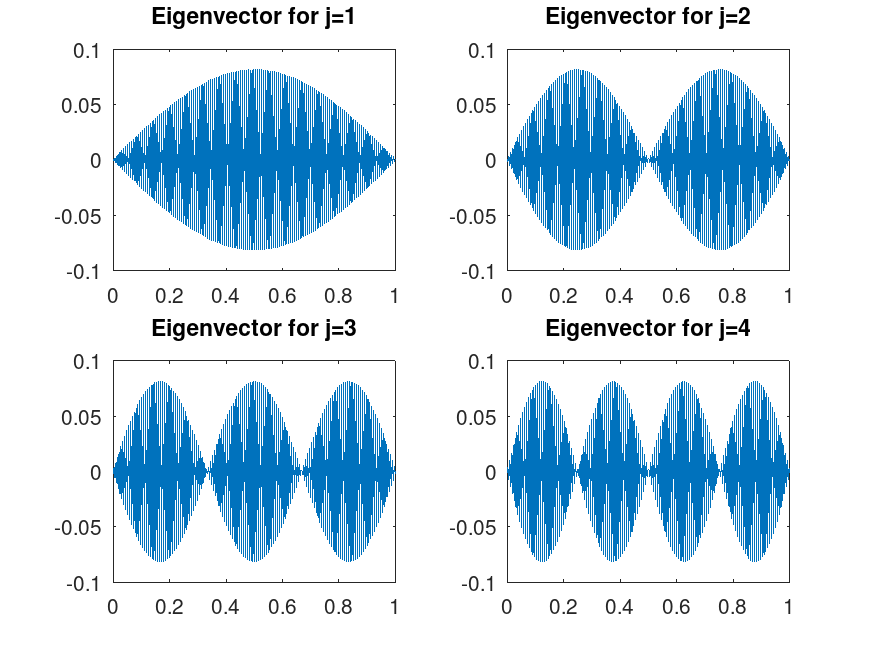
\includegraphics[width=0.80\textwidth]{problem_1a_eigenvectors.png}
        \caption{Eigenvectors for 1D eigenvalue Dirichlet BVP}
    \end{figure}
\end{solution}